% CRS CataLyst-5 trajectory platform architecture
% Compile with pdfLaTeX. Requires TikZ.
\documentclass[tikz,border=8pt]{standalone}
\usepackage[T1]{fontenc}
\usepackage{tikz}
\usetikzlibrary{arrows.meta,positioning,fit}
\begin{document}
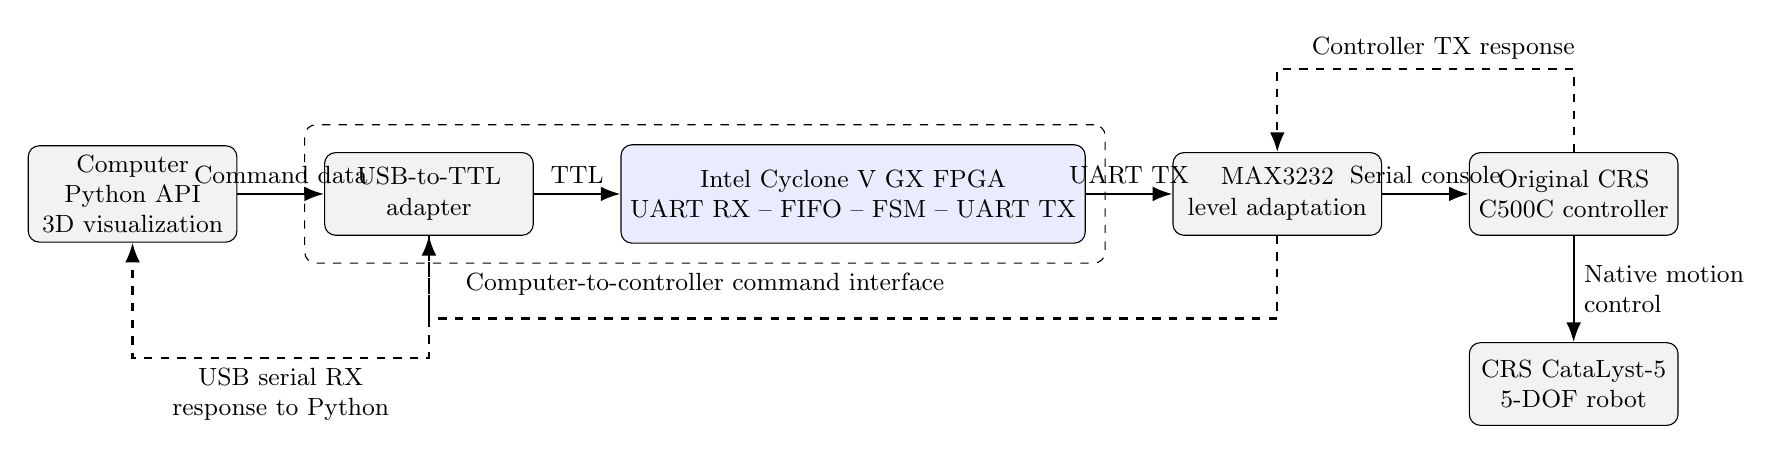
\begin{tikzpicture}[
  font=\small,
  block/.style={draw,rounded corners,align=center,minimum width=2.65cm,minimum height=1.05cm,fill=gray!10},
  fpga/.style={draw,rounded corners,align=center,minimum width=3.15cm,minimum height=1.25cm,fill=blue!8},
  forward/.style={-{Latex[length=2.5mm]},thick},
  response/.style={-{Latex[length=2.5mm]},thick,dashed}
]
\node[block] (pc) {Computer\\Python API\\3D visualization};
\node[block,right=1.1cm of pc] (usb) {USB-to-TTL\\adapter};
\node[fpga,right=1.1cm of usb] (fpga) {Intel Cyclone V GX FPGA\\UART RX -- FIFO -- FSM -- UART TX};
\node[block,right=1.1cm of fpga] (max) {MAX3232\\level adaptation};
\node[block,right=1.1cm of max] (ctrl) {Original CRS\\C500C controller};
\node[block,below=1.35cm of ctrl] (robot) {CRS CataLyst-5\\5-DOF robot};

\draw[forward] (pc) -- node[above,align=center] {Command data} (usb);
\draw[forward] (usb) -- node[above] {TTL} (fpga);
\draw[forward] (fpga) -- node[above] {UART TX} (max);
\draw[forward] (max) -- node[above,align=center] {Serial console} (ctrl);
\draw[forward] (ctrl) -- node[right,align=left] {Native motion\\control} (robot);

% Response path: controller to computer, bypassing the FPGA.
\draw[response] (ctrl.north) -- ++(0,1.05) -| node[pos=0.22,above,align=center] {Controller TX response} (max.north);
\draw[response] (max.south) -- ++(0,-1.05) -| (usb.south);
\draw[response] (usb.south) -- ++(0,-1.55) -| node[pos=0.25,below,align=center] {USB serial RX\\response to Python} (pc.south);

\node[draw,dashed,rounded corners,fit=(usb)(fpga),inner sep=7pt,label=below:{Computer-to-controller command interface}] {};
\end{tikzpicture}
\end{document}
